\section{示例:一級標題}
\subsection{示例:二級標題}
\subsubsection{示例:三級標題}
(1) 此部分是論文之主體,包括研究方法、設計以及資料之收集、處理,
分析和討論。

(2) 能清楚地描述取樣對象及方法,範圍和性質,運用合適的研究工具,
詳細交待研究的實施程序,有初步性探討,以確定研究方法及程序
之可行性,並提供詳盡的研究記錄和資料。

(3) 正確、清楚及合理地將資料整理,交待和分析。客觀而無偏見地引
述文獻於討論和分析中,明確列舉研究發現,且提示與先前相關研
究發現之異同,明確區分事實與推論,而不致混淆。統計圖表的應
用適當而且清楚。

(4) 論文的主要觀點在此部分應得到充分的論證,包括理論和實踐 (即案
例)兩個部分。

(5)論證章的資料收集:資料收集的描述應達到科學研究的清晰和重複
性的要求;資料收集的描述包括研究主體,觀測方法和觀測過程。

(6)論證章的資料處理:描述統計、頻率分析、資料變換、X2 分析、
圖表用來表示分析的結果等。

(7)論證章的資料分析:闡明所採用的資料分析方法,應用此方法分析
計算的結果以及此結果的統計顯著性;統計顯著性才能驗證假設的
真偽。忌諱花大量的篇幅去講述分析方法的原理和步驟,或論文只
交代採用什麼方法和得出的結果,而資料分析過程無交代。

(8)論證章寫作要點:論證章的標題應反映出該章所論證的假設,才能
顯現出研究的文獻;清楚研究物件和研究情境的定位,圍繞假設向
深處、細處展開;知識性內容越少越好。忌諱按照教科書的思路,
似乎在告訴讀者這方面的知識,而看不出研究的貢獻何在。

\subsection{示例:數學公式}
公式:式子置中,編號(\ref{eq1})(第2章,第1個公式)靠右,如
\begin{equation}
\label{eq1}
	e^{\pi i}+1=0
\end{equation}


\subsection{示例:插圖格式要求}
圖:居中,圖的標題在圖的下方,編號以圖 1-1(第一章第一個圖)表示,
以後的圖按順序排列, 圖 \ref{fig:sig}, 圖 1-3…; 圖 3-1 (第三章第一個圖)等等。
\subsubsection{圖示例:單標題單圖}
\par 單標題單圖示例:
\begin{figure}[H]
	\centering
	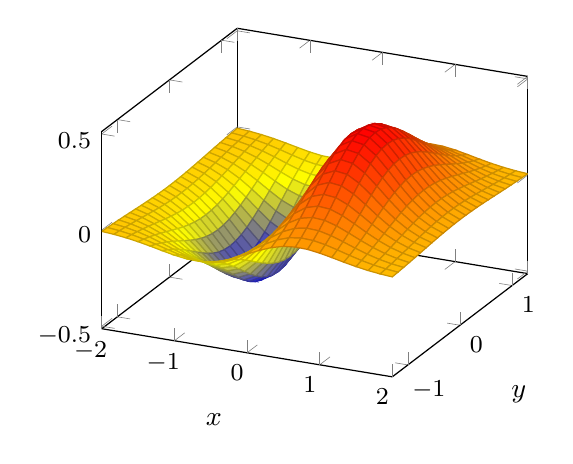
\begin{tikzpicture}[scale=1.1]
	\begin{axis}[
	xlabel=$x$, ylabel=$y$,
	small,
	]
	\addplot3 [
	surf,
	domain=-2:2,
	domain y=-1.3:1.3,
	] {exp(-x^2-y^2)*x};
	\end{axis}
	\end{tikzpicture}
	\caption{$x\cdot \exp(-x^2-y^2)$ 函數圖}
	\label{fig:sig}
\end{figure}
圖\ref{fig:sig}表示$x\cdot \exp(-x^2-y^2)$ 函數圖.



\subsubsection{圖示例:單標題多子圖}
\par 一標題多子圖示例

\tikzstyle{every pin}=[fill=white,draw=black,font=\small,]
\begin{figure}[H]
	\centering
	\begin{subfigure}{.49\textwidth}
	  	\centering
		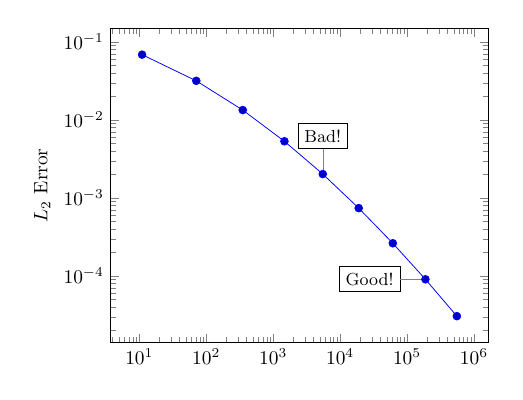
\begin{tikzpicture}[scale=0.7]
			\begin{loglogaxis}[
				%xlabel={\textsc{Dof}},
				ylabel={$L_2$ Error},
				]
				\addplot coordinates {
					(11, 6.887e-02)
					(71, 3.177e-02)
					(351, 1.341e-02)
					(1471, 5.334e-03)
					(5503, 2.027e-03)
					(18943, 7.415e-04)
					(61183, 2.628e-04)
					(187903, 9.063e-05)
					(553983, 3.053e-05)
				};
				\node [coordinate,pin=above:{Bad!}]
				at (axis cs:5503,2.027e-03) {};
				\node [coordinate,pin=left:{Good!}]
				at (axis cs:187903,9.063e-05) {};
			\end{loglogaxis}
		\end{tikzpicture}
		\caption{A subfigure}
		\label{fig:sub1}
	\end{subfigure}
	\begin{subfigure}{.49\textwidth}
		\centering
		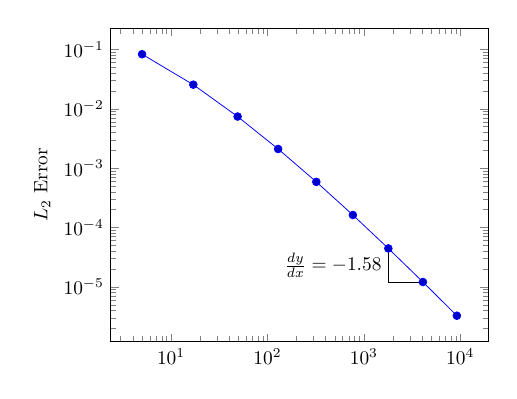
\begin{tikzpicture}[scale=0.7]
			\begin{loglogaxis}[
				ylabel=$L_2$ Error,
				]
				\draw
				(1793,4.442e-05)
				|- (4097,1.207e-05)
				node [near start,left]
				{$\frac{dy}{dx} = -1.58$};
				\addplot coordinates {
					(5, 8.312e-02)
					(17, 2.547e-02)
					(49, 7.407e-03)
					(129, 2.102e-03)
					(321, 5.874e-04)
					(769, 1.623e-04)
					(1793, 4.442e-05)
					(4097, 1.207e-05)
					(9217, 3.261e-06)
				};
			\end{loglogaxis}
		\end{tikzpicture}
		\caption{A subfigure}
	  	\label{fig:sub2}
	\end{subfigure}\\

	\begin{subfigure}{.49\textwidth}
		\centering
		
\includegraphics[width=.5\linewidth]{figure/eg05}
		\caption{A subfigure}
		\label{fig:sub3}
	\end{subfigure}
	\begin{subfigure}{.49\textwidth}
		\centering
		
\includegraphics[width=.5\linewidth]{figure/eg06}
		\caption{A subfigure}
		\label{fig:sub4}
	\end{subfigure}
	\caption{A figure with two subfigures}
	\label{fig:sub}
\end{figure}
	
	
上面示例中,子圖\ref{fig:sub1}、子圖\ref{fig:sub2}、子圖\ref{fig:sub3}、子圖\ref{fig:sub4}分別表示子圖

	
	
\subsubsection{圖示例:多標題多圖}
\par 多標題多圖示例
\begin{figure}[H]
	\centering
	\begin{minipage}{.48\textwidth}
		\centering

		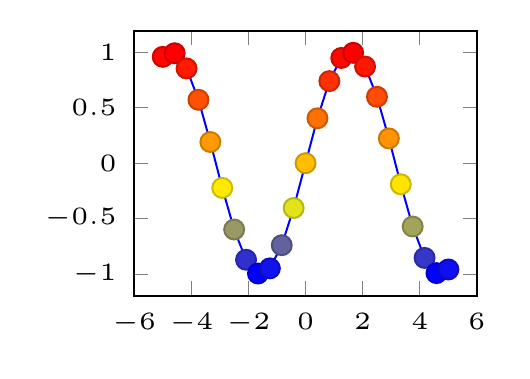
\begin{tikzpicture}[scale=1.8]
		\begin{axis}[tiny]
		\addplot+ [scatter] {sin(deg(x))};
		\end{axis}
		\end{tikzpicture}

		\captionof{figure}{A figure}
		\label{fig:test1}
	\end{minipage}%
	\begin{minipage}{.48\textwidth}
		\centering
		
		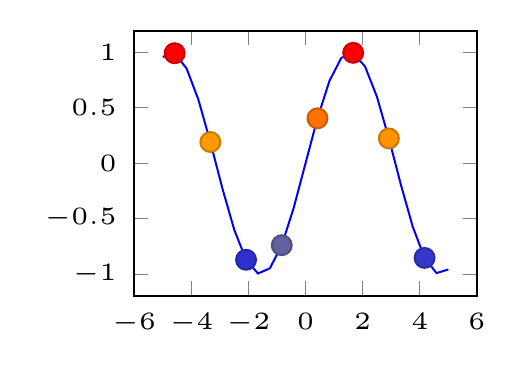
\begin{tikzpicture}[scale=1.8]
		\begin{axis}[tiny]
		\addplot+ [scatter,
		mark repeat=3,mark phase=2]
		{sin(deg(x))};
		\end{axis}
		\end{tikzpicture}
			
		\captionof{figure}{Another figure}
		\label{fig:test2}
	\end{minipage}
\end{figure}
上面示例中,圖\ref{fig:test1}、圖\ref{fig:test2}分別表示兩張獨立的圖


\subsection{示例:表格格式要求}
\par 表:居中,表的標題在表格的上方,編號以“表 2-1”(第二章第一個表)表
示,以後的表按順序排列,表\ref{tab:t1},表 2-2;表 3-1(第三章第一個表)以此類推。


\begin{table}[H]	
	\centering
	\caption{示例正常小表}
	\begin{tabular}[l]{@{}lcccccc}		
		\toprule		
		Class$^{\rm a}$ & $\gamma_1$ & $\gamma_2$$^{\rm b}$& $\langle \gamma \rangle$& $G$ & $|{ f}|$ & $\theta _{c}$ \\		
		\midrule	
		BL Lacs &5 & 36 & 7 & $-4.0$ & $1.0\times 10^{-2}$ & 10$^\circ$ \\		
		FSRQs & 5 & 40 & 11 & $-2.3$ & $0.5\times 10^{-2}$ & 14$^\circ$ \\		
		\bottomrule		
	\end{tabular}
	\label{tab:t1}
\end{table}

下面是一張超長表
\begin{sidewaystable}[!htp]
	
	\caption{示例旋轉長表} 
	\centering
	\setlength{\tabcolsep}{10mm}
	\begin{tabular}[l]{@{}lcccccc}		
	\toprule		
	Class$^{\rm a}$ & $\gamma_1$ & $\gamma_2$$^{\rm b}$& $\langle \gamma \rangle$& $G$ & $|{ f}|$ & $\theta _{c}$ \\		
	\midrule	
	BL Lacs &5 & 36 & 7 & $-4.0$ & $1.0\times 10^{-2}$ & 10$^\circ$ \\		
	FSRQs & 5 & 40 & 11 & $-2.3$ & $0.5\times 10^{-2}$ & 14$^\circ$ \\		
	\bottomrule		
\end{tabular}
\end{sidewaystable}


$\mathfrak{fer}$














